\documentclass{standalone}
\usepackage{tikz}
\usetikzlibrary{calc}
\tikzset{%
  add/.style args={#1 and #2}{
    to path={%
      ($(\tikztostart)!-#1!(\tikztotarget)$)--($(\tikztotarget)!-#2!(\tikztostart)$)%
      \tikztonodes},add/.default={.2 and .2}}
}


\tikzset{%
  mark coordinate/.style={inner sep=0pt,outer sep=0pt,minimum size=3.5pt,
    fill=black,circle}%
}

\newcommand\pgfmathsinandcos[3]{%
  \pgfmathsetmacro#1{sin(#3)}%
  \pgfmathsetmacro#2{cos(#3)}%
}
\newcommand\LongitudePlane[2][current plane]{%
  \pgfmathsinandcos\sinEl\cosEl{\Elevation} % elevation
  \pgfmathsinandcos\sint\cost{#2} % azimuth
  \tikzset{#1/.estyle={cm={\cost,\sint*\sinEl,0,\cosEl,(0,0)}}}
}
\newcommand\LatitudePlane[2][current plane]{%
  \pgfmathsinandcos\sinEl\cosEl{\Elevation} % elevation
  \pgfmathsinandcos\sint\cost{#2} % latitude
  \pgfmathsetmacro\ydelta{\cosEl*\sint}
  \tikzset{#1/.estyle={cm={\cost,0,0,\cost*\sinEl,(0,\ydelta)}}} %
}
\newcommand\DrawLongitudeCircle[1]{
  \LongitudePlane{#1}
  \tikzset{current plane/.prefix style={scale=\R}}
  \pgfmathsetmacro\angVis{atan(sin(#1)*cos(\Elevation)/sin(\Elevation))} %
  \draw[current plane,dashed] (\angVis-180:1) arc (\angVis-180:\angVis:1);
  \draw[current plane]  (\angVis:1)     arc (\angVis:\angVis+180:1);
}%

\newcommand\DrawLatitudeCircle[1]{
  \LatitudePlane{#1}
  \tikzset{current plane/.prefix style={scale=\R}}
  \pgfmathsetmacro\sinVis{sin(#1)/cos(#1)*sin(\Elevation)/cos(\Elevation)}
  \pgfmathsetmacro\angVis{asin(min(1,max(\sinVis,-1)))}
  \draw[current plane, dashed] (180-\angVis:1) arc (180-\angVis:\angVis:1);
  \draw[current plane] (\angVis:1) arc
  (\angVis:-\angVis-180:1);
  % \node () at (5,3) {\angVis};
}%

\newcommand\DrawPointOnSphere[3]{%
  \pgfmathsinandcos\sinLoM\cosLoM{#1}
  \pgfmathsinandcos\sinLaM\cosLaM{#2}
}


\begin{document}
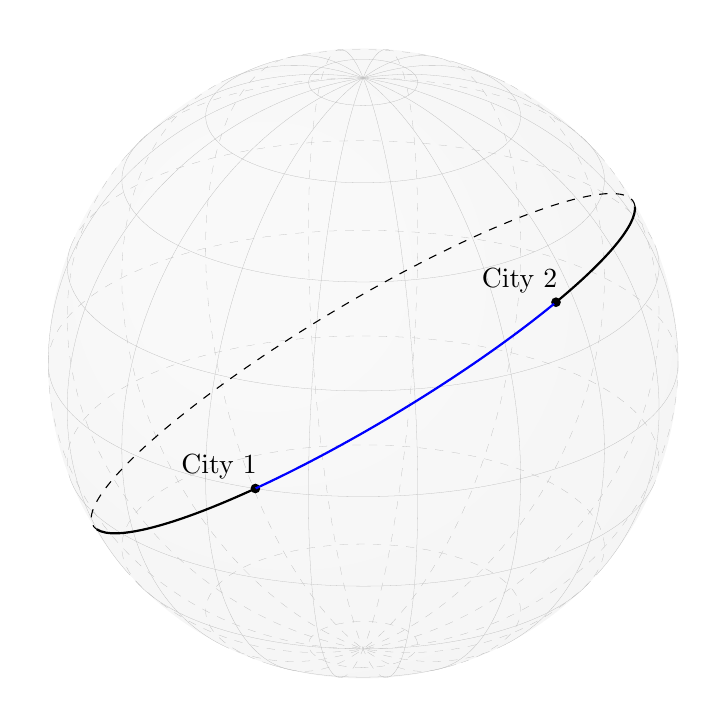
\begin{tikzpicture}
  \def\R{4} % sphere radius
  \def\Elevation{25} % elevation angle
  \def\angleLongitudeP{-110} % longitude of point P
  \def\angleLongitudeQ{-45} % longitude of point Q
  \def\angleLatitudeQ{30} % latitude  Q    ; 0 latitude of P
  \def\angleLongitudeA{-20} % longitude of point A

  \pgfmathsetmacro\H{\R*cos(\Elevation)} % distance to north pole
  \LongitudePlane[PLongitudePlane]{\angleLongitudeP}
  \LongitudePlane[QLongitudePlane]{\angleLongitudeQ}
  \LongitudePlane[ALongitudePlane]{\angleLongitudeA}

  % \begin{scope}[opacity=.05]                   %
  \fill[ball color=white, opacity=.025] (0,0) circle (\R); % 3D lighting effect
  % \end{scope}
  \coordinate (O) at (0,0);
  \coordinate[] (N) at (0,\H);
  \coordinate[] (S) at (0,-\H);

  \begin{scope}[every path/.style={ultra thin, gray!50!white}]
    \foreach \myangle in {-80, -60, ..., 80}{
      \DrawLatitudeCircle{\myangle} % Latitude
    }
    % \DrawLatitudeCircle{100} % Latitude
    \foreach \myangle in {20, 40, ..., 180}{
      \DrawLongitudeCircle{\myangle} % Latitude
    }
  \end{scope}

  % \DrawLatitudeCircle{10}

  % \DrawLongitudeCircle{\angleLongitudeP} % PLongitudePlane
  % \DrawLongitudeCircle{\angleLongitudeQ} % QLongitudePlane
  % \DrawLongitudeCircle{\angleLongitudeA}
  % \DrawLatitudeCircle{\angleLatitudeQ}
  % \DrawLatitudeCircle{0} % equator
  % \DrawLongitudeCircle{0}
  % setup coordinates P and Q
  % \path[ALongitudePlane] (0:\R) coordinate (A);
  \path[ALongitudePlane] (32.5:\R) coordinate (A');
  \path[ALongitudePlane] (122.5:\R) coordinate (N');
  \path[PLongitudePlane] (0:\R) coordinate (P);
  % \draw[dashed,add= 1 and 0] (O) to  (P);
  \path[QLongitudePlane] (\angleLatitudeQ:\R) coordinate (Q);
  % \draw[dashed,add= 1 and 0] (O) to  (Q) ;
  \path[QLongitudePlane] (0:\R) coordinate (B);
  % \draw [dashed] (O) --  (B) ;
  % \draw [dashed] (O) --  (N) ;

  \foreach \v/\l in {P/City 1,Q/City 2} {\coordinate[mark coordinate] (v) at (\v);
    \node [above left, xshift=4pt] at (\v) {\l};}
  \begin{scope}[ x={(P)}, y={(A')}, z={(N')}]
    \draw[dashed,fill opacity=.3] circle (1);
    \draw[thick, blue] ( 0:1) arc (0:68:1) ;
    \draw[thick] ( 68:1) arc (68:115:1) ;
    \draw[thick] (-55:1) arc (-55:0:1);
    % \draw[red,->](0,0,0)--(Q);
    % \draw[red,->](0,0,0)--(0,1,0);
    % \draw[red,->](0,0,0)--(1,0,0);
  \end{scope}
  % \coordinate[mark coordinate] (origin) at (0,0);
  % \node[above] at (origin) {origin};

\end{tikzpicture}

\end{document}
